%-----------------------------------------------------
% Chapter: Methodology
%-----------------------------------------------------
\chapter{Methodology}
This chapter describes the methodology used during this project. 
\label{chap:data_methodology}
\section{Collecting Data}
As previously mentioned, a central repository for song lyrics, where downloading is permissive, is non-existent. Collection of song lyrics from sites such as Genius\footnote{https://genius.com/} is only achievable through web scraping: a process which involves the exhaustive downloading and processing of web pages from either a predefined list of URLs or the recursive process of link extraction and following (commonly known as \textit{web crawling}) from a given seed URL. When scraping at scale, restrictions such as the robots exclusion protocol, which specifies areas of a website that are allowed to be processed, and crawl rate, which specifies the minimum delay between requests, make data collection via this method a troublesome task. Taking into account the project aims and constraints such as time, web scraping was deemed unfavourable and hence avoided for data collection.

\noindent
\newline
To fulfil the data requirements of the project, a public dataset \footnote{https://www.kaggle.com/neisse/scrapped-lyrics-from-6-genres} containing over 250,000 song lyrics was used. The dataset, which was scraped from Brazilian music website Vagalume.br, comprised of two \textit{.csv} files: artists-data and lyrics-data. The artist-data file included metrics such as popularity, genre and number of songs per artist, whilst the lyrics-data file contained song lyrics for individual songs by artists.

\section{Data Analysis and Restructuring}
The CoVeR algorithm requires each document within a corpus to be associated with a covariate in order to jointly learn word embeddings and the relevant transformation matrices. To satisfy this requirement, Pandas, a Python data analysis library, was used to perform a join operation on the artists columns in both the artists-data and lyrics-data files. The result of this operation followed by the additional dropping of redundant columns resulted in the dataset used throughout the rest of the project.

\noindent
\newline
(IMAGE OF DATASET SCHEMA)

\noindent
\newline
A trivial approach to divide the dataset on genre would involve an equal split for equal representation, however, this method has the assumption that for each genre, word count per song is equivalent. Examining the dataset however, proved this not to be the case.
\begin{figure}[h]
	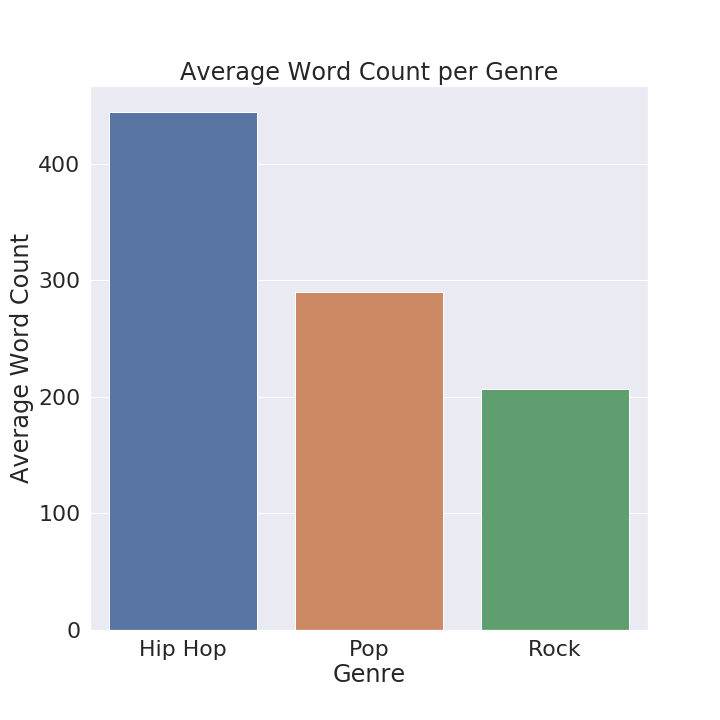
\includegraphics[width=8cm, height=8cm]{./figures/fig6}
	\centering
	\caption{Average word count per lyric per genre in the dataset}
	\label{fig:fig6}
\end{figure}

\noindent
\newline
Analysing the dataset, the mean number of words contained in a Hip Hop song was 444; being more than double the mean number of words found in Rock songs, which had a count of 207. With regards to the Pop genre, the mean word count per song was 289. To reflect these statistics and also due to constraints in the distribution of data by genre, 100,000 song lyrics were randomly selected to create the dataset to be used to train CoVeR. Moreover, a data split of 48:30:22 for Rock, Pop and Hip-Hop, was to maintain an even distribution of words by song genre within the dataset.
\section{Data Pre-processing}
Essential to any machine learning task is the pre-processing of input data in such a way that important features are accessible during training. In NLP, this can include techniques such as tokenisation, string cleaning, stemming and lemmatisation.

\noindent
\newline
Following reconstructing of the original dataset, each song lyric in the dataset was cleansed and tokenised. The following string cleaning techniques were applied to each song lyric.

\begin{enumerate}
	\item All characters, except for letters, were substituted with a space.
	\item All letters were lowercased.
	\item All text between curly and square brackets were removed. (This was to ensure text like \textbf{[Verse 1]} was not included during training).
	\item All trailing white space was removed.
\end{enumerate}

\noindent
\newline
Tokenisation is the process of separating textual inputs into meaningful chunks called \textit{tokens}. Naturally to create word embeddings, text is tokenised at the word level and each token is assigned a unique integer key to map the token to its future word embedding.

\section{Hyperparameters}
In machine learning hyperparameters are parameters that govern a given model. The selection of these parameters directly impacts the performance of a given training algorithm and as such, hyperparameter choice is important for producing optimal performance for a given model. Commonly, techniques such as grid search, random search and manual search are used to find optimal optimal parameters for a given training algorithm. However, due to the time constraints of this project, hyperparameter search, especially in the case of fine tuning LSTM's, was limited.

\noindent
\newline
Both CoVeR and LSTM networks have important hyperparameters which are reviewed in the following sections
\subsection{CoVeR Hyperparamters}
\subsubsection{Removing Rare Words}
Word embedding methods such as word2vec typically remove rare occurring words within a corpus before training takes place. In the case of word2vec, rare words are removed, \textit{before} the computation of co-occurrence statistics. This method of removal has the effect of generating  context windows differing to the context windows generated from the original corpus. In turn this produces differing \(i,j\) co-occurrences. This is highlighted in the example below.

\noindent
\newline
Sentence: Fly me to the moon.
\noindent
\newline
Context of "to" (without removal of rare words): me, the
\noindent
\newline
Context of "to" (with removal of rare words): Fly, moon

\noindent
\newline
Neither the CoVeR or GloVe paper, discuss the removal of rare words, however many implementations (REF) 
\subsubsection{Subsampling}
Typically found within text corpora are high frequency stop words which provide less information than rarely occurring words (\cite{Mikolov2013a}). For example This concept can also be applied to word embeddings; where the word embeddings of frequent words does not change significantly after training on several examples. Taking inspiration from word2vec, subsampling was used at the covariate level using the following adapted formula from the original word2vec implementation.

\begin{equation}
P(w_{ik}) = \sqrt{\dfrac{z(w_{ik})}{t}} + 1 \cdot \dfrac{t}{z(w_{ik})}
\end{equation}

\noindent
\newline
where \(z(w_{ik})\) is the percentage of word \(w_{ik}\) in covariate \(k\) and \(t\) is a chosen threshold.
\subsubsection{Context Windows}
CoVeR uses the same weighted context windows strategy as GloVe during the process of calculating co-occurrence statistics. The CoVeR paper uses a context window size of 8, however the paper does not specify whether they used symmetric or asymmetric windows during their experiments. As such, both are experimented with whilst performing hyperparameter tuning.  
\subsubsection{Embedding Size}
\subsubsection{Optimiser}
\subsubsection{Tuning}
\subsection{LSTM Hyperparameters}
\subsubsection{Dropout}
Dropout is a regularization technique proposed by \cite{Srivastava2014}, which involves the random dropping of nodes and their connections within a network. Selected nodes are picked at random using a probability known as the dropout rate. Dropout helps to decrease over-fitting as 
\subsubsection{Embedding Layer}
For both the language model and the text classifier, the first layer of the network is the embedding layer which transforms words, represented as indices, into word embeddings. They can either be initialised randomly as one-hot vectors and trained with the network or they can be initialised using pre trained word embeddings, which can either be left as is or trained further. For this project the word embeddings learnt from cover were used as the initialiser for the embedding layer, and after initial experiments were allowed to be trained.
\subsubsection{Optimiser}

